% Provenance (never printed): see sources/outline_sources.md (Year 1: heat sources,
% radiogenic and secular cooling; heat-flow measurement; the steady conductive geotherm
% with heat production; convection against conduction; the lithosphere as a thermal
% boundary layer). Curves from figdata/bachelor-1/geotherms.py; exercise and problem
% values in the Book 3 scratch calculator calc/ch10.py.
\chapter{地球的热收支}\label{ch:b1:heat-budget}

在日本阿尔卑斯山下的一处旧矿洞里，一个装有千吨液体闪烁体的罐子
正在等待微弱的闪光。大多数闪光来自周围国家核反应堆产生的
反中微子，但也有一些来自地下：地球内部的铀和钍在衰变时
放出反中微子，这些反中微子
穿过整个地球，
仿佛地球中空无一物。在 2135 天的计数中，探测器共记录到 841 个候选事件，
其中 106 个被归因于地球本身。从这少量闪光中，
其研究团队于 2011 年估计，铀和钍的衰变以约 20 太瓦的功率加热地球。
地球整体散失的热量约为 47 太瓦。本章说明这一差额：
地球热量从何而来，流出的热量如何测量，
热量以传导方式传递时温度如何随深度升高，
为什么\omterm{def:b1:layered-earth:layers}{地幔}必须对流，
以及为什么板块是这种对流的冷上边界。

\begin{recall}
热量从高温流向低温；岩石的热导率 $k$ 表示热量穿过岩石的难易程度，
热扩散率 $\kappa = k/(\rho c)$ 表示温度变化扩散的快慢（物理学，本科二年级）。
放射性原子核以固定的半衰期衰变（物理学）。沿\omterm{def:b1:heat-budget:geotherm}{地温线}，
温度随深度升高，\omterm{def:b1:layered-earth:layers}{地幔}发生对流（第 2 册，十一和十二年级）。
\omterm{def:b1:layered-earth:lithosphere}{岩石圈}是地球坚硬的外壳，
（见\cref{ch:b1:layered-earth}）。
\end{recall}

\section{热量从何而来}

\begin{definition}[热流]\label{def:b1:heat-budget:heat-flow}
地球表面某点处的\emph{热流}\index{热流} $q$，即表面热流密度，
是指该处穿过地表的内部起源功率，按单位面积计，
取向外为正。其单位为
\unit{W.m^{-2}}，实际中常用 \unit{mW.m^{-2}}。对整个地表积分，
即得地球的热损失 $Q = \oint q\,\mathrm dS$。
\end{definition}

\omterm{def:b1:heat-budget:heat-flow}{热流}已在数万个地点测得。2010 年发表的汇编
收录了 \num{38347} 个测量值，给出下列平均值，
其中海洋与大陆分别统计：
\begin{center}
\small
% ledger: dd10:split, dd10:total
\begin{tabular}{lccc}
\hline
 & 面积（\unit{m^2}） & 热损失（\unit{TW}） & 平均\omterm{def:b1:heat-budget:heat-flow}{热流}（\unit{mW.m^{-2}}） \\
\hline
大陆 & \num{2.073e14} & 14.7 & 70.9 \\
海洋 & \num{3.028e14} & 31.9 & 105.4 \\
整个地球 & \num{5.101e14} & 46.7 & 91.6 \\
\hline
\end{tabular}
\end{center}
总量经不确定度取整后为 $Q = \qty[uncertainty-mode=separate]{47 \pm 2}{TW}$。其中三分之二
经由洋底散失，洋底比
大陆年轻且更薄。这是一股很小的\omterm{def:b1:heat-budget:heat-flow}{热流}：太阳输送给地球的能量约为 \qty{173000}{TW}，
地球，地球内部热量约为
地表能量收支的 \qty{0.03}{\percent}。 % ledger: nasa:solar-mean
但正是这股\omterm{def:b1:heat-budget:heat-flow}{热流}驱动着火山、板块运动和造山作用，它
有两个来源。

\begin{definition}[放射性生热]\label{def:b1:heat-budget:heat-production}
岩石的\emph{放射性生热}\index{放射性生热} $A$，是指
单位体积、单位时间内，其所含放射性原子核衰变所释放的热量，
单位为 \unit{W.m^{-3}}，实际中常用
\unit{\micro W.m^{-3}}。设岩石密度为 $\rho$，
其中产热元素的质量分数为 $C_i$，各元素每千克释放 $H_i$ 瓦特热量，
则有
\[
  A = \rho \sum_i C_i H_i .
\]
\end{definition}

四种同位素产生了几乎全部的这部分热量，因为它们寿命长、
丰度足够高且能量足够大：\ce{^{238}U}、\ce{^{235}U}、\ce{^{232}Th} 和
\ce{^{40}K}。每种元素每千克的热量，等于其放射性同位素每千克的热量
乘以该同位素在元素中所占的份额
（见\cref{exo:b1:heat-budget:3}）：
\begin{center}
\small
% ledger: dye:isotope-heat, iaea:isotopes
\begin{tabular}{lcccc}
\hline
同位素 & 半衰期 & 每千克同位素的热量 & 元素中的 & 每千克元素的热量 \\
 & （\unit{Ga}） & （\unit{W.kg^{-1}}） & 占比（按原子数） & （\unit{W.kg^{-1}}） \\
\hline
\ce{^{238}U} & 4.468 & \num{9.513e-5} & \qty{99.274}{\percent} & U: \num{9.85e-5} \\
\ce{^{235}U} & 0.704 & \num{5.685e-4} & \qty{0.720}{\percent} & \\
\ce{^{232}Th} & 14.0 & \num{2.628e-5} & 几乎全部 & Th: \num{2.63e-5} \\
\ce{^{40}K} & 1.248 & \num{2.847e-5} & \qty{0.0117}{\percent} & K: \num{3.40e-9} \\
\hline
\end{tabular}
\end{center}
钾每千克释放的热量比铀少约三万倍，
但钾是许多岩石中的主要元素，其含量以百分比计，
而铀和钍的含量以百万分之一计。三者含量都高的岩石是
花岗岩及其近缘岩石；含量最低的是\omterm{def:b1:layered-earth:layers}{地幔}橄榄岩。另有
对 \num{2188} 项分析结果的汇编给出以下中位数，单位为 \unit{\micro
W.m^{-3}}:
\begin{center}
\small
% ledger: vila:heat-production
\begin{tabular}{lclclc}
\hline
流纹岩 & 2.55 & 泥质岩 & 1.44 & 辉长岩 & 0.35 \\
花岗岩 & 2.43 & 砂岩 & 0.82 & 玄武岩 & 0.21 \\
花岗闪长岩 & 1.88 & 碳酸盐岩 & 0.42 & 超镁铁质岩 & 0.11 \\
\hline
\end{tabular}
\end{center}
各组内部的差异很大：四分之一的花岗岩产热低于
\qty{1.74}{\micro W.m^{-3}}，四分之一的花岗岩产热高于 \qty{3.23}{\micro W.m^{-3}}。
大陆\omterm{def:b1:layered-earth:layers}{地壳}富集这些元素，洋壳和
\omterm{def:b1:layered-earth:layers}{地幔}则相对贫化；但\omterm{def:b1:layered-earth:layers}{地幔}体积极大，
仍占有地球热源的很大份额。

\begin{definition}[长期冷却]\label{def:b1:heat-budget:secular-cooling}
\emph{长期冷却}\index{长期冷却}是地球热损失中由地球内部、\omterm{def:b1:layered-earth:layers}{地幔}和地核
的温度缓慢下降所提供的部分，即自行星形成以来所储存热量的释放，
其速率为
$-\sum_j M_j c_j\,\mathrm dT_j/\mathrm dt$，
其中 $M_j$ 为各储库的质量，$c_j$ 为比热，$T_j$ 为平均温度。
\end{definition}

能量守恒给出了整个地球的热量收支：
地表散失的热量等于\omterm{def:b1:heat-budget:heat-production}{放射性生热}与\omterm{def:b1:heat-budget:secular-cooling}{长期冷却}之和，
\[
  Q = H_{\text{放射}} + Q_{\text{长期}} .
\]
地中微子测量了第一项的一部分：2011 年的结果综合了两台探测器，
将 \qty{20}{TW} 归于铀和钍，以及
\ce{^{40}K} 的反中微子太弱，无法以此方式探测，
已知其约贡献 \qty{4}{TW}。
% ledger: kamland:2011
因此，约一半的热损失来自\omterm{def:b1:heat-budget:heat-production}{放射性生热}，另一半，
约 \qty{23}{TW}，属于\omterm{def:b1:heat-budget:secular-cooling}{长期冷却}。其中一部分冷却来自地核：
穿过\omterm{def:b1:layered-earth:discontinuity}{核幔边界}的热量估计为 \qtyrange{5}{15}{TW}。
这些数值并不确定：测量本身带有约
\qty{9}{TW} 的不确定度，而迄今的地中微子结果只把放射性部分限定在
\qtyrange{15}{41}{TW} 之间，而不同类型的地球模型则给出
\qtyrange{14}{46}{TW} 的分布范围。在地表测得的总量，
是收支中最为可靠的一项（见下图）。
% ledger: dye:radiogenic

\begin{omfigure}
\begin{tikzpicture}[x=0.24cm, y=1cm, font=\small]
% ledger: dd10:split, kamland:2011, dye:radiogenic
% losses
\fill[blue!22] (0,1.6) rectangle (31.9,2.3);
\fill[brown!35] (31.9,1.6) rectangle (46.6,2.3);
\draw (0,1.6) rectangle (46.6,2.3);
\draw (31.9,1.6) -- (31.9,2.3);
\node at (15.95,1.95) {海洋 31.9};
\node at (39.25,1.95) {大陆 14.7};
\node[anchor=east, align=right, font=\small] at (-0.5,1.95) {地表 \\散失};
% sources
\fill[orange!35] (0,0) rectangle (20,0.7);
\fill[yellow!45] (20,0) rectangle (24,0.7);
\fill[red!18] (24,0) rectangle (46.7,0.7);
\draw (0,0) rectangle (46.7,0.7);
\draw (20,0) -- (20,0.7) (24,0) -- (24,0.7);
\node at (10,0.35) {U 和 Th 20};
\node at (22,0.35) {K 4};
\node at (35.35,0.35) {长期冷却 $\approx 23$};
\node[anchor=east, align=right] at (-0.5,0.35) {热源};
% core part of secular cooling (range)
\draw[red!60!black, very thick] (24,-0.25) -- (29,-0.25);
\draw[red!60!black, thick, densely dashed] (29,-0.25) -- (39,-0.25);
\draw[red!60!black] (24,-0.15) -- (24,-0.35) (39,-0.15) -- (39,-0.35);
\node[anchor=north, font=\scriptsize, red!60!black] at (31.5,-0.3) {穿过核幔边界的热量，\qtyrange{5}{15}{TW}};
% radiogenic range
\draw[|-|, orange!70!black, thick] (15,1.0) -- (41,1.0);
\node[anchor=south, font=\scriptsize, orange!70!black] at (28,1.02) {放射性估计范围，\qtyrange{15}{41}{TW}};
% axis
\draw[->] (0,-1.05) -- (50,-1.05) node[right] {TW};
\foreach \x in {0,10,20,30,40} {\draw (\x,-1.0) -- (\x,-1.1) node[below, font=\scriptsize] {\x};}
\end{tikzpicture}

\par\smallskip{\small 地球的热量收支。上：通过洋底和大陆散失的热量，
共 \qty[uncertainty-mode=separate]{47 \pm 2}{TW}。下：其热源，
其中铀和钍的放射性部分由地中微子测量，
钾的部分由估计得出；其余部分由差减得到，即\omterm{def:b1:heat-budget:secular-cooling}{长期冷却}，其中
地核所提供的部分尚不清楚。橙色条表示
地中微子测量所允许的放射性部分的范围。}
\label{fig:b1:heat-budget:budget}
\end{omfigure}

过去\omterm{def:b1:heat-budget:heat-production}{放射性生热}更大，因为同位素的丰度更高：
\ce{^{235}U} 和 \ce{^{40}K}，即短寿命的那几种，当时的贡献要大得多
（第 2 册，十二年级）。地球的热机正在缓慢减弱，
两方面都如此。

\section{测量热流}

\omterm{def:b1:heat-budget:heat-flow}{热流}不是直接测量的：它由温度梯度
和热导率计算得出。

\begin{proposition}[傅里叶定律]\label{prop:b1:heat-budget:fourier}
在热导率为 $k$ 的介质中，热量沿温度梯度
下降的方向传导，传导速率与梯度成正比（按单位面积计）。设 $z$ 为深度
（向下为正），$q$ 为\omterm{def:b1:heat-budget:heat-flow}{热流}（向上为正），则
\[
  q = k\,\frac{\mathrm dT}{\mathrm dz} .
\]
\end{proposition}
\admitted

该定律已在物理系列的本科二年级分册中确立。
大多数岩石在低于
\qty{200}{\celsius} 时的热导率为 \qtyrange{1.5}{3}{W.m^{-1}.K^{-1}}，温度越高则越小；大陆\omterm{def:b1:heat-budget:heat-flow}{热流}模型
给出花岗质上\omterm{def:b1:layered-earth:layers}{地壳}的热导率约为 \qty{2.7}{W.m^{-1}.K^{-1}}；
% ledger: delaney:conductivity, roy:granitic-k
若其中温度梯度为 \qty{25}{K.km^{-1}}，则\omterm{def:b1:heat-budget:heat-flow}{热流}约为
\qty{70}{mW.m^{-2}}。

当钻孔穿过的岩石热导率不同时，
梯度在相邻岩层之间发生变化，而\omterm{def:b1:heat-budget:heat-flow}{热流}不变，只要
它们之间没有热量产生或储存。下面的命题将此转化为
一个检验。

\begin{proposition}[布拉德图]\label{prop:b1:heat-budget:bullard}
设 $R(z) = \int_0^z \mathrm d\zeta/k(\zeta)$ 为单位面积上的
地表至深度 $z$ 之间岩石的热阻，单位为
\unit{m^2.K.W^{-1}}。若\omterm{def:b1:heat-budget:heat-flow}{热流} $q$ 在钻孔各深度处都相同，
则温度是热阻的线性函数：
$T(z) = T_0 + q\,R(z)$。
\end{proposition}

\begin{proof}
由傅里叶定律，$\mathrm dT/\mathrm dz = q/k(z)$。从 $0$ 积分到
$z$，且 $q$ 为常数，$T(z) - T_0 = q\int_0^z \mathrm d\zeta/k(\zeta) = q\,R(z)$。
\end{proof}

\begin{method}[由钻孔测定热流]\label{met:b1:heat-budget:borehole}
\begin{enumerate}
  \item 钻孔完成很久之后，待钻井液的扰动已消失，
        再沿钻孔测量温度，并舍去最浅的数十米，
        其温度随季节变化。
  \item 在实验室测量所穿过的每种岩石岩芯的热导率，
        并在每个记录深度上计算
        热阻 $R(z)$。
  \item 以 $T$ 对 $R$ 作图：直线的斜率即为\omterm{def:b1:heat-budget:heat-flow}{热流}。
        曲线的弯折说明岩层中有水流动、地表温度曾发生变化，
        或热导率存在误差。
  \item 必要时进行修正：地形使等温线在丘陵与山谷之下弯曲；
        末次冰期以来的缓慢变暖仍影响上部约一千米，
        同样需要修正。
\end{enumerate}
\end{method}

在海上不需要钻孔。深海海底的温度非常稳定，
因此只需数米厚的软沉积物，便已达到平衡梯度。
将一根携带一排温度传感器的钢制探杆从船上放下，
借助重物将其打入沉积物中（见下图）；
传感器记录梯度，
并沿探杆发送一个热脉冲，即可就地测得沉积物的热导率。
洋底存在一个陷阱。在年轻的洋壳上，海水在破裂的玄武岩中循环，
并通过平流带走大部分热量，
所测得的传导\omterm{def:b1:heat-budget:heat-flow}{热流}远小于真实的热损失。
因此，最年轻洋底的热损失须由
\cref{sec:b1:heat-budget:boundary-layer}中的冷却模型计算，该模型
在循环已停止的老洋壳上标定：这一计算部分，
\qty{23.1}{TW}，约占全球总量的一半。% ledger: dd10:young-ocean

\begin{omfigure}
\begin{tikzpicture}[font=\scriptsize, x=1cm, y=1cm]
% --- left: borehole on land ---
\fill[brown!12] (0,0) rectangle (3.2,-1.6);
\fill[red!10] (0,-1.6) rectangle (3.2,-4.2);
\draw[thick] (0,0) -- (3.2,0);
\node[anchor=west] at (0.05,-0.8) {页岩，$k$ 低};
\node[anchor=west] at (0.05,-2.9) {花岗岩，$k$ 高};
\draw[black!60] (0,-1.6) -- (3.2,-1.6);
\draw[very thick] (2.5,0.3) -- (2.5,-4.0);
\draw[gray] (2.5,0.6) -- (2.5,0.3);
\foreach \y in {-0.6,-1.2,-1.8,-2.4,-3.0,-3.6} {\fill[red!70!black] (2.5,\y) circle (1.6pt);}
\node[anchor=south] at (2.5,0.6) {温度测井};
% inset T(z)
\draw[->] (3.7,0) -- (5.6,0) node[right] {$T$};
\draw[->] (3.7,0) -- (3.7,-4.2) node[below] {$z$};
\draw[thick, red!70!black] (3.9,-0.1) -- (4.9,-1.6) -- (5.4,-4.0);
\node[anchor=west, align=left] at (4.9,-1.0) {页岩中 \\较陡};
\node[anchor=west, align=left] at (5.25,-3.0) {花岗岩中 \\较缓};
\node[anchor=north] at (2.6,-4.45) {(a) 钻孔：各岩层中 $q = k\,\mathrm dT/\mathrm dz$};
% --- right: probe at sea ---
\begin{scope}[xshift=8.6cm]
\fill[blue!8] (0,0) rectangle (5.4,-2.6);
\draw[blue!50, thick] (0,0) .. controls (0.6,0.08) and (1.2,-0.08) .. (1.8,0)
  .. controls (2.4,0.08) and (3.0,-0.08) .. (3.6,0) .. controls (4.2,0.08) and (4.8,-0.08) .. (5.4,0);
\fill[gray!60] (1.6,0.02) -- (3.0,0.02) -- (2.8,0.3) -- (1.8,0.3) -- cycle;
\node[anchor=south] at (2.3,0.32) {船};
\draw[gray] (2.4,0.02) -- (2.4,-2.75);
\fill[brown!25] (0,-2.6) rectangle (5.4,-4.2);
\draw (0,-2.6) -- (5.4,-2.6);
\node[anchor=west] at (3.0,-3.0) {软沉积物};
\node[anchor=west] at (3.0,-3.4) {（数米）};
\fill[black!70] (2.2,-2.75) rectangle (2.6,-3.0);
\draw[very thick] (2.4,-3.0) -- (2.4,-4.0);
\foreach \y in {-3.2,-3.45,-3.7,-3.95} {\fill[red!70!black] (2.4,\y) circle (1.6pt);}
\node[anchor=east, align=right] at (2.1,-2.85) {重物};
\node[anchor=east, align=right] at (2.25,-3.55) {带传感器 \\的探杆};
\node[anchor=west] at (0.1,-1.3) {深水，温度稳定};
\node[anchor=north] at (2.7,-4.45) {(b) 海上：将探杆打入沉积物};
\end{scope}
\end{tikzpicture}

\par\smallskip{\small \omterm{def:b1:heat-budget:heat-flow}{热流}测量（示意图，未按比例）。(a) 在陆地上，
温度在钻孔中恢复到平衡后沿钻孔测量，每种岩石的热导率
在岩芯上测得：岩层的梯度在热导率较低处较陡，
而\omterm{def:b1:heat-budget:heat-flow}{热流}（即梯度与热导率之积）处处相同。
(b) 在海上，带传感器的探杆被打入洋底沉积物中，
深度为数米。}
\label{fig:b1:heat-budget:measure}
\end{omfigure}

\begin{inthefield}[海上测热流]
\begin{minipage}[t]{0.55\linewidth}\vspace{0pt}
在科学考察船上，\omterm{def:b1:heat-budget:heat-flow}{热流}探杆是一根由船尾吊车悬挂的沉重探杆。
它借船上的缆绳放至刚好位于海底上方，随后松开：
重物将其打入沉积物，船员在甲板上等待传感器
恢复到泥的温度，再将探杆提起，驶向不远处的下一个测站。
沿洋脊侧翼排列的一排测站，
可显示\omterm{def:b1:heat-budget:heat-flow}{热流}随海底年龄的衰减；
相邻测站之间的离散性说明水
在何处流过下方的\omterm{def:b1:layered-earth:layers}{地壳}。
\end{minipage}\hfill
\begin{minipage}[t]{0.42\linewidth}\vspace{0pt}
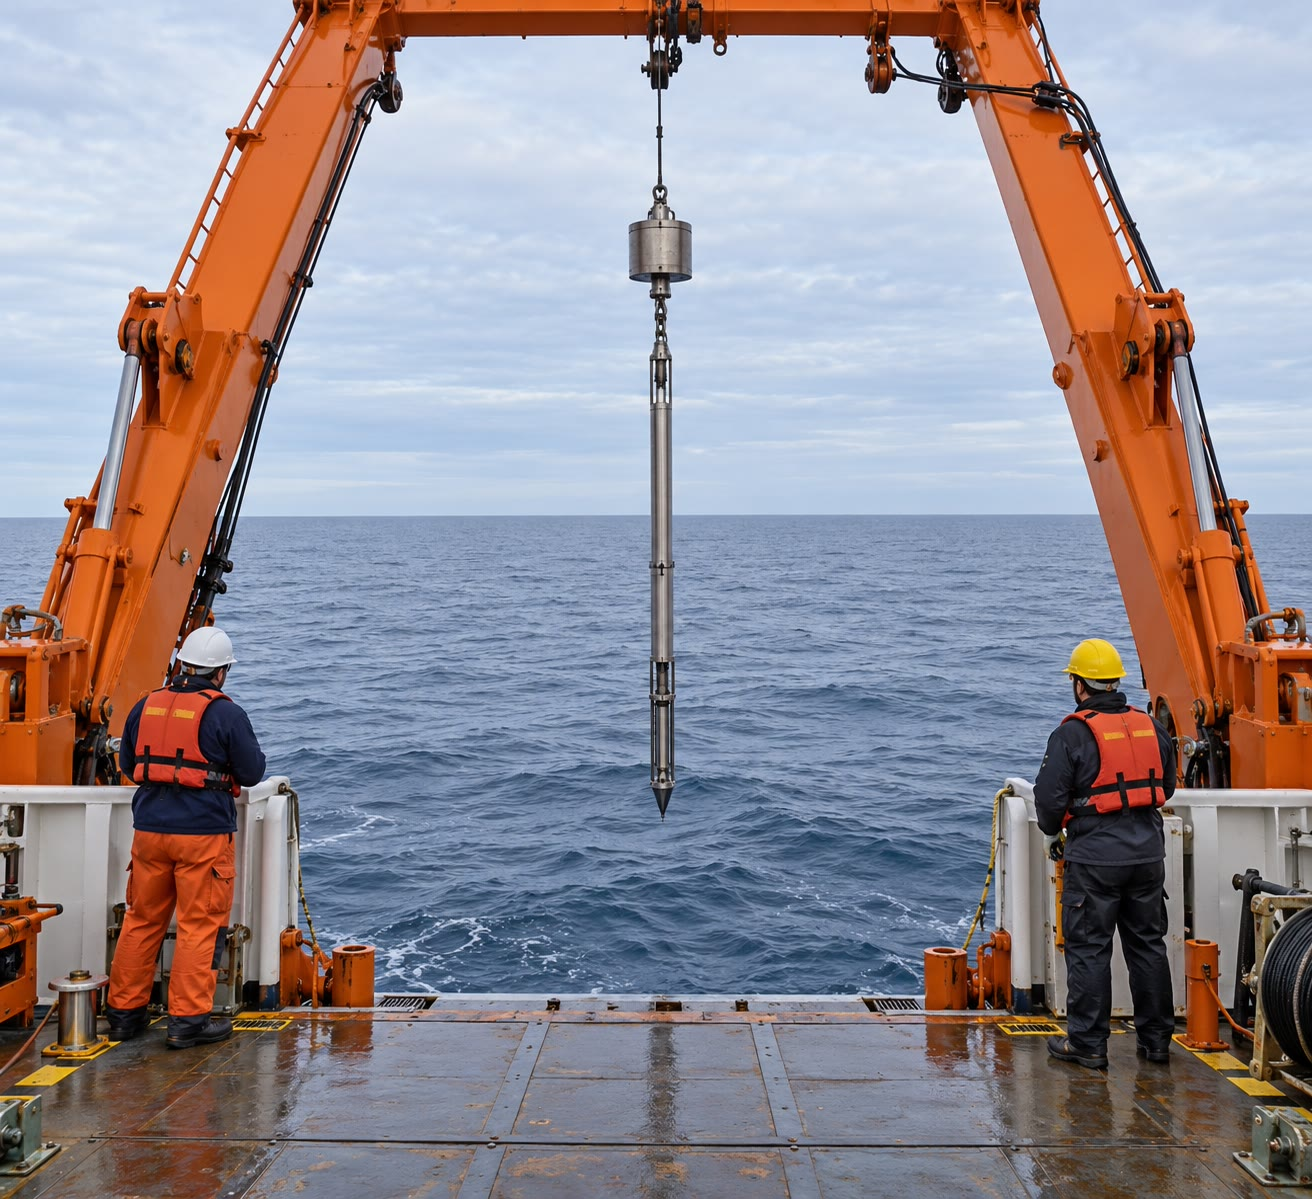
\includegraphics[width=\linewidth]{images/book3/ai/b1-heatflow-probe.jpg}

{\scriptsize 悬挂于科学考察船船尾吊车上的\omterm{def:b1:heat-budget:heat-flow}{热流}探杆
（AI 生成插图）。}
\end{minipage}
\end{inthefield}

\section{稳态传导地温线}

\begin{definition}[地温线]\label{def:b1:heat-budget:geotherm}
地表某点之下的\emph{地温线}\index{地温线}，即该处温度随深度的变化，
$T(z)$。若其不随时间变化，
且热量仅通过传导沿其传递，
则称之为稳态传导地温线。
\end{definition}

远离活火山和水循环的\omterm{def:b1:layered-earth:lithosphere}{岩石圈}内，
热量以传导方式输运，在数百万年的尺度上
\omterm{def:b1:heat-budget:geotherm}{地温线}是稳定的。其形状于是由能量平衡决定。

\begin{theorem}[有生热的稳态传导]\label{thm:b1:heat-budget:balance}
沿稳态传导\omterm{def:b1:heat-budget:geotherm}{地温线}，在导热率 $k$ 均匀的介质中，
生热率为 $A(z)$，且热量无水平流动，则
\[
  \frac{\mathrm dq}{\mathrm dz} = -A(z), \qquad\text{即}\qquad
  k\,\frac{\mathrm d^2T}{\mathrm dz^2} = -A(z).
\]
\end{theorem}

\begin{proof}
考虑面积为 $S$ 的水平薄板，位于深度 $z$ 与 $z +
\mathrm dz$ 之间。热量从其底面以速率 $q(z + \mathrm dz)\,S$ 流入，
从顶面以速率 $q(z)\,S$ 流出，内部产生热量的速率为
$A(z)\,S\,\mathrm dz$。稳态下热量不积累，故
$q(z)\,S = q(z + \mathrm dz)\,S + A(z)\,S\,\mathrm dz$，由此得
$\mathrm dq/\mathrm dz = -A$。由傅里叶定律 $q = k\,\mathrm dT/\mathrm dz$，
且 $k$ 为常数，故 $k\,T'' = -A$。
\end{proof}

自地表向下看，\omterm{def:b1:heat-budget:heat-flow}{热流}随深度递减，递减量等于
其上方各层产生的热量：穿过地表的热量即来自
下方的热量加上沿途产生的全部热量。$A$ 的两种分布给出
闭式解。

\begin{proposition}[均匀放射性层]\label{prop:b1:heat-budget:uniform}
设生热率 $A$ 自地表向下直至深度 $h$，在其以下为零，
地表温度为 $T_0$，地表\omterm{def:b1:heat-budget:heat-flow}{热流}为 $q_0$。
则当 $0 \le z \le h$ 时，
\[
  q(z) = q_0 - A z, \qquad T(z) = T_0 + \frac{q_0 z}{k} - \frac{A z^2}{2k},
\]
在 $h$ 以下\omterm{def:b1:heat-budget:heat-flow}{热流}均匀，$q_m = q_0 - A h$，\omterm{def:b1:heat-budget:geotherm}{地温线}为
斜率为 $q_m/k$ 的直线。
\end{proposition}

\begin{proof}
由 $\mathrm dq/\mathrm dz = -A$ 从 $0$ 起积分，以 $q(0) = q_0$ 为初值，得 $q = q_0 -
Az$。于是 $\mathrm dT/\mathrm dz = (q_0 - Az)/k$；以 $T(0) = T_0$ 积分，
得抛物线。在 $h$ 以下，$\mathrm dq/\mathrm dz = 0$，$q$ 保持其
在 $h$ 处的值。
\end{proof}

\begin{theorem}[指数型生热率与线性热流关系]
\label{thm:b1:heat-budget:exponential}
设生热率随深度按 $A(z) = A_0 e^{-z/D}$ 递减，\omterm{def:b1:heat-budget:heat-flow}{热流}
在极大深度处趋于 $q_m$，地表温度为 $T_0$。则
\[
  q(z) = q_m + A_0 D\,e^{-z/D}, \qquad
  T(z) = T_0 + \frac{q_m z}{k} + \frac{A_0 D^2}{k}\bigl(1 - e^{-z/D}\bigr),
\]
且地表\omterm{def:b1:heat-budget:heat-flow}{热流}为
\[
  q_0 = q_m + A_0 D .
\]
\end{theorem}

\begin{proof}
由\cref{thm:b1:heat-budget:balance}，$\mathrm dq/\mathrm dz =
-A_0e^{-z/D}$，故 $q(z) = A_0 D e^{-z/D} + C$；当 $z \to \infty$ 时 $q \to C$，
因此 $C = q_m$。在 $z = 0$ 处，$q_0 = q_m + A_0 D$。于是 $\mathrm dT/\mathrm dz =
q/k = q_m/k + (A_0D/k)\,e^{-z/D}$，自 $0$ 起积分并取 $T(0) = T_0$，
得 $T = T_0 + q_m z/k + (A_0 D^2/k)(1 - e^{-z/D})$。
\end{proof}

最后一行是一个可在地表检验的预测。同一地区的花岗岩深成岩体
共享相同的深部\omterm{def:b1:heat-budget:heat-flow}{热流} $q_m$；若它们仅在铀、钍、钾的含量上有差别，
则其特征尺度 $D$ 也相同。于是，在每个深成岩体上测得的\omterm{def:b1:heat-budget:heat-flow}{热流}
应是其岩石中测得的生热率的线性函数，
斜率为 $D$（一个长度），
截距为 $q_m$，即来自放射性层之下的约化\omterm{def:b1:heat-budget:heat-flow}{热流}。
弗朗西斯·伯奇于 1968 年首次观测到这样的直线，
同年他依据这些直线划分了三个地质省：
\begin{center}
\small
% ledger: roy:provinces, roy:linear-relation
\begin{tabular}{lcc}
\hline
地质省 & 截距 $q_m$（\unit{mW.m^{-2}}） & 斜率 $D$（\unit{km}） \\
\hline
美国东部 & 33 & 7.5 \\
盆岭省 & 59 & 9.4 \\
内华达山脉 & 17 & 10 \\
\hline
\end{tabular}
\end{center}
截距原以 0.8、1.4 和 $0.4\times\qty{e-6}{cal.cm^{-2}.s^{-1}}$ 发表，
按 $\qty{1}{\micro cal.cm^{-2}.s^{-1}} = \qty{41.84}{mW.m^{-2}}$ 换算
（见\cref{exo:b1:heat-budget:4}）。斜率变化很小，从 7 到 \qty{10}{km}；约化\omterm{def:b1:heat-budget:heat-flow}{热流}
变化很大，其分布图显示下方\omterm{def:b1:layered-earth:layers}{地幔}何处较热，例如
盆岭省伸展\omterm{def:b1:layered-earth:layers}{地壳}之下。
\cref{prop:b1:heat-budget:uniform} 中的均匀层也给出一条直线，斜率为 $h$：
两种模型都能拟合数据，但只有指数模型
在深成岩体被剥蚀至不同深度时仍保持相同斜率的直线
（见\cref{exo:b1:heat-budget:10}），因此更受青睐。

\begin{omfigure}
\begin{tikzpicture}
\begin{axis}[omdepth, width=0.82\linewidth, height=8.6cm, xmin=0, xmax=1800, ymin=0, ymax=250, axis x line=top, axis y line=left, axis line style={-}, clip=true,
  xlabel={温度（\unit{\degreeCelsius}）}, ylabel={深度（km）},
  tick label style={font=\scriptsize}, label style={font=\small},
  legend style={font=\scriptsize, at={(0.02,0.02)}, anchor=south west, draw=none, fill=white, fill opacity=0.85, text opacity=1},
  legend cell align=left]
\addplot[very thick, black!45] table[x=T, y=depth] {figdata/out/bachelor-1-geotherms-adiabat.dat};
\addlegendentry{地幔绝热线}
\addplot[very thick, red!75!black] table[x=T45, y=depth] {figdata/out/bachelor-1-geotherms-continental.dat};
\addlegendentry{$q_0 = \qty{70}{mW.m^{-2}}$}
\addplot[very thick, orange!80!black] table[x=T30, y=depth] {figdata/out/bachelor-1-geotherms-continental.dat};
\addlegendentry{$q_0 = \qty{55}{mW.m^{-2}}$}
\addplot[very thick, green!45!black] table[x=T15, y=depth] {figdata/out/bachelor-1-geotherms-continental.dat};
\addlegendentry{$q_0 = \qty{40}{mW.m^{-2}}$}
\addplot[thick, blue!70!black, densely dashdotted] table[x=T, y=depth] {figdata/out/bachelor-1-geotherms-oceanic.dat};
\addlegendentry{海底，\qty{60}{Ma} 龄}
\addplot[thin, dashed, red!75!black, forget plot] table[x=Tc45, y=depth] {figdata/out/bachelor-1-geotherms-continental.dat};
\addplot[thin, dashed, orange!80!black, forget plot] table[x=Tc30, y=depth] {figdata/out/bachelor-1-geotherms-continental.dat};
\addplot[thin, dashed, green!45!black, forget plot] table[x=Tc15, y=depth] {figdata/out/bachelor-1-geotherms-continental.dat};
\draw[densely dotted, black!60] (axis cs:0,35) -- (axis cs:1800,35);
\node[font=\scriptsize, anchor=south east] at (axis cs:1790,35) {莫霍面，\qty{35}{km}};
\fill (axis cs:1384.0,70.8) circle (1.6pt);
\fill (axis cs:1403.2,107.8) circle (1.6pt);
\fill (axis cs:1459.7,224.9) circle (1.6pt);
\node[font=\scriptsize, anchor=west] at (axis cs:1420,66) {\qty{71}{km}};
\node[font=\scriptsize, anchor=west] at (axis cs:1440,104) {\qty{108}{km}};
\node[font=\scriptsize, anchor=west] at (axis cs:1495,222) {\qty{225}{km}};
\end{axis}
\end{tikzpicture}

\par\smallskip{\small 大陆的稳态传导\omterm{def:b1:heat-budget:geotherm}{地温线}，其生热
率 $A_0 = \qty{2.5}{\micro W.m^{-3}}$ 在 $D = \qty{10}{km}$ 的深度范围内递减，
$k = \qty{2.5}{W.m^{-1}.K^{-1}}$，对应三种地表\omterm{def:b1:heat-budget:heat-flow}{热流}（折算\omterm{def:b1:heat-budget:heat-flow}{热流}
15、30 和 \qty{45}{mW.m^{-2}}）。每条曲线沿其传导曲线（虚线部分为外推）
向下延伸至\omterm{def:b1:heat-budget:adiabat}{地幔绝热线}，并在圆点处与之相交，即\omterm{def:b1:heat-budget:boundary-layer}{热
岩石圈}的底部。洋底\omterm{def:b1:heat-budget:geotherm}{地温线}为冷却
\qty{60}{Ma} 的半空间的\omterm{def:b1:heat-budget:geotherm}{地温线}。传导率均匀仅为一种简化。}
\label{fig:b1:heat-budget:geotherms}
\end{omfigure}

\begin{method}[深成岩体之下的温度]\label{met:b1:heat-budget:moho}
\begin{enumerate}
  \item 在深成岩体上方测量地表\omterm{def:b1:heat-budget:heat-flow}{热流} $q_0$（钻孔法），
        并由其 U、Th 和 K 含量求出生热率 $A_0$。
  \item 取该省的\omterm{def:b1:heat-budget:heat-flow}{热流}线，或取 $D$ 约为
        \qty{10}{km}，计算 $q_m = q_0 - A_0 D$。
  \item 应用\cref{thm:b1:heat-budget:exponential}。在 $D$ 的数倍以下，
        $e^{-z/D}$ 可忽略，\omterm{def:b1:heat-budget:geotherm}{地温线}即为直线
        $T_0 + A_0D^2/k + q_m z/k$：放射性层使各深处的温度都
        升高了 $A_0D^2/k$。
\end{enumerate}
\end{method}

图中，\omterm{def:b1:layered-earth:discontinuity}{莫霍面}处的温度范围是：\omterm{def:b1:heat-budget:heat-flow}{热流}最低时约为 \qty{320}{\degreeCelsius}，
\omterm{def:b1:heat-budget:heat-flow}{热流}最高时超过 \qty{700}{\degreeCelsius}：地表\omterm{def:b1:heat-budget:heat-flow}{热流}直接给出了深部\omterm{def:b1:layered-earth:layers}{地壳}的
温度读数，而该温度决定了其强度
（见\cref{ch:b1:stress-strain-rheology}）。

\section{传导与对流}

传导很慢。其慢到何种程度，由热传导方程可以看出，该方程
由物理学教材依据傅里叶定律及
\cref{thm:b1:heat-budget:balance}中的平衡关系（加上储热项）推导而来：一维情形下，
无生热时，
$\partial T/\partial t = \kappa\,\partial^2 T/\partial z^2$。

\begin{proposition}[传导时间尺度]\label{prop:b1:heat-budget:timescale}
在导热体边界上施加的温度变化，会扩散至
距离 $L$ 处，所需时间的量级为：
\[
  \tau = \frac{L^2}{\kappa} .
\]
\end{proposition}

\begin{proof}
令 $z = L z^*$，$t = \tau t^*$，其中 $z^*$ 与 $t^*$ 均为无量纲的。热
传导方程化为 $\partial T/\partial t^* = (\kappa\tau/L^2)\,\partial^2
T/\partial z^{*2}$。其解在 $z^* \sim 1$ 的尺度上、$t^* \sim 1$ 时发生变化，
仅当系数量级为一，即 $\tau \sim L^2/\kappa$ 时，此式才成立。
\end{proof}

岩石的热扩散率 $\kappa \approx \qty{e-6}{m^2.s^{-1}}$。日温度循环
可深入地下数十厘米，年温度循环可深入数米，而
自上一次冰期以来的升温则深达约一千米。对于\omterm{def:b1:layered-earth:lithosphere}{岩石圈}，
其厚 \qty{100}{km}，$\tau = \qty{e16}{s}$，约 \qty{300}{Ma}。对于
厚 \qty{2900}{km} 的\omterm{def:b1:layered-earth:layers}{地幔}，$\tau = \qty{8.4e18}{s}$，即 \qty{270}{Ga}，
为地球年龄 \qty{4.54}{Ga} 的六十倍。% ledger: england:kelvin, usgs:age-earth
仅靠传导，深部\omterm{def:b1:layered-earth:layers}{地幔}的热量不可能被带到
地表附近。\omterm{def:b1:layered-earth:layers}{地幔}发生对流，其内部的热量由
岩石自身的运动携带，速度与板块相当，约为每
年数厘米。% ledger: usgs:san-andreas

\begin{definition}[地幔绝热线]\label{def:b1:heat-budget:adiabat}
\emph{地幔绝热线}\index{地幔绝热线}是对流\omterm{def:b1:layered-earth:layers}{地幔}的
充分混合内部的\omterm{def:b1:heat-budget:geotherm}{地温线}：\omterm{def:b1:layered-earth:layers}{地幔}岩石上升或下沉时
速度足够快而与外界不交换热量，其所取的温度
即为该\omterm{def:b1:heat-budget:geotherm}{地温线}，上升时因膨胀而冷却，
下沉时因压缩而升温。
\end{definition}

由热力学可得其梯度 $\mathrm dT/\mathrm dz = \alpha g T/c_p$，
其中 $\alpha$ 为热膨胀系数，$c_p$ 为比热容（物理学内容，
此处在本阶段不加证明地承认）。该梯度很小。一项近期的\omterm{def:b1:rock-forming-minerals:mineral}{矿物}物理学评估给出
在 \qty{50}{km} 深度处为 \qty{0.54}{K.km^{-1}}，降至 \qty{0.36}{K.km^{-1}}
于 \qty{410}{km} 处，随后在下\omterm{def:b1:layered-earth:layers}{地幔}中由 0.41 降至 \qty{0.23}{K.km^{-1}}，
其温度在 \qty{50}{km} 处为 \qty{1646}{K}，在 \qty{2800}{km} 处为 \qty{2587}{K}。
% ledger: katsura:adiabat
将绝热线外推至地表，即得\omterm{def:b1:layered-earth:layers}{地幔}的位温
\qty{1619}{K}，约 \qty{1350}{\degreeCelsius}：即\omterm{def:b1:layered-earth:layers}{地幔}在不与外界交换热量的前提下
被带至地表时所具有的温度。位温的概念，对于大气与
海洋，其定义见
\cref{ch:b1:fluid-envelopes-structure}。温度每千米仅升高
\qty{0.5}{K}，而近地表的传导\omterm{def:b1:heat-budget:geotherm}{地温线}每千米升高
\qty{25}{K}，这正是对流的特征。

\begin{history}[约翰·佩里与冷却的地球]
1862--1863 年间，后来被封为开尔文勋爵的汤姆孙，
通过地球的冷却计算了地球年龄。他将地球视为固体，其热量经传导，
自约 \qty{3900}{\degreeCelsius} 的均匀温度冷却下来；
他依当时的测量所取的平均梯度约为
\qty{36}{K.km^{-1}}，热扩散率取
\qty{1.2e-6}{m^2.s^{-1}}，则达到今日梯度所需的时间约为
\qty{96}{Ma}，其范围介于 24 与 \qty{400}{Ma} 之间（见\cref{exo:b1:heat-budget:9}）。地质学家
认为此结果过短。1895 年，
即放射性被发现的前一年，他的前助手约翰·佩里
转而指出一项假设：若内部部分为流体并发生对流，
则其传热如同具有极大传导率一般，而整个内部
而非薄薄的外壳，都将为地表\omterm{def:b1:heat-budget:heat-flow}{热流}供热。佩里的论证
被忽视并遗忘；此后确立的\omterm{def:b1:layered-earth:layers}{地幔}对流证明了他是对的：
深部\omterm{def:b1:layered-earth:layers}{地幔}以对流方式冷却，这正是预算中的
\omterm{def:b1:heat-budget:secular-cooling}{长期冷却}。% ledger: england:kelvin, england:perry
\end{history}

\begin{proposition}[佩里的充分混合地球]\label{prop:b1:heat-budget:perry}
设半径为 $R$ 的球体内部充分混合，温度均匀为
$T_i(t)$，单位体积热容为 $\rho c$，位于
厚度为 $L \ll R$、传导率为 $k$ 的导热盖层之下，其表面
温度为 $\qty{0}{\degreeCelsius}$，且无生热。则
\[
  T_i(t) = T_i(0)\,e^{-t/\tau_P}, \qquad \tau_P = \frac{RL}{3\kappa},
\]
且地表\omterm{def:b1:heat-budget:heat-flow}{热流} $kT_i/L$ 以相同的时间常数衰减。
\end{proposition}

\begin{proof}
由于盖层很薄，它处于稳态，并输运\omterm{def:b1:heat-budget:heat-flow}{热流}
$q = kT_i/L$。内部通过面积 $4\pi R^2$ 散失热量：
$\tfrac43\pi R^3\rho c\,\mathrm dT_i/\mathrm dt = -4\pi R^2 kT_i/L$，即
$\mathrm dT_i/\mathrm dt = -3\kappa T_i/(RL)$，其中 $\kappa = k/(\rho c)$，其解
为时间常数为 $\tau_P = RL/(3\kappa)$ 的指数函数。
\end{proof}

设 $R = \qty{6400}{km}$，$L = \qty{100}{km}$，$\kappa =
\qty{e-6}{m^2.s^{-1}}$，则 $\tau_P = \qty{6.8}{Ga}$。对流的地球
能长达数十亿年保持较高的\omterm{def:b1:heat-budget:heat-flow}{热流}，而开尔文设想的导热地球
则在数千万年内便失去了这一\omterm{def:b1:heat-budget:heat-flow}{热流}（见\cref{exo:b1:heat-budget:11}）。

\section{作为热边界层的岩石圈}\label{sec:b1:heat-budget:boundary-layer}

\begin{definition}[热边界层，热岩石圈]\label{def:b1:heat-budget:boundary-layer}
在对流流体中，\emph{热边界层}\index{热边界层}是沿某一边界分布的一层，
热量借传导穿过该层，
温度由边界处的值变为充分混合内部的值。
\emph{热岩石圈}\index{热岩石圈}是\omterm{def:b1:layered-earth:layers}{地幔}的上部热边界层，
即地球由地表向下直至
传导\omterm{def:b1:heat-budget:geotherm}{地温线}与\omterm{def:b1:heat-budget:adiabat}{地幔绝热线}相交的深度处
的外壳。
\end{definition}

板块是\omterm{def:b1:layered-earth:layers}{地幔}对流的冷顶，即其上部边界层。
板块的底部，即陡峭的传导\omterm{def:b1:heat-budget:geotherm}{地温线}转为平缓的
绝热线之处，位于\omterm{def:b1:heat-budget:geotherm}{地温线}图所示的 \qtyrange{70}{230}{km} 深处，
对应大陆\omterm{def:b1:heat-budget:heat-flow}{热流} 70 至 \qty{40}{mW.m^{-2}}，深度落在地震学测定的范围内
（见\cref{ch:b1:layered-earth}）：由强度定义的\omterm{def:b1:layered-earth:lithosphere}{岩石圈}
与由温度定义的\omterm{def:b1:layered-earth:lithosphere}{岩石圈}大体上是同一壳层，
因为强度取决于温度。在\omterm{def:b1:layered-earth:layers}{地幔}底部，
D$''$ 层是下部边界层，由地核自下方加热。

在大洋下方，边界层形成于洋脊处，那里热的\omterm{def:b1:layered-earth:layers}{地幔}上升至地表，
并随板块远离洋脊而逐渐冷却增厚。
由均匀温度出发的半空间冷却问题，经傅里叶求解、开尔文用于整个地球，
很好地描述了这一过程（见\cref{ch:b1:rifts-ridges-margins}
及本科三年级分册推导）：等温线深度随海底年龄的
平方根增加（见下图），\omterm{def:b1:heat-budget:heat-flow}{热流}随时间按
如下规律减小：
\[
  q(t) = \frac{C}{\sqrt t}, \qquad C \approx \qty{490}{mW.m^{-2}.Ma^{1/2}},
\]
即全球热收支中所用的数值。 % ledger: dd10:young-ocean
在 \qty{100}{Ma} 时，半空间已冷却至约 \qty{130}{km} 深（见\cref{exo:b1:heat-budget:12}）。实际板块更早停止增厚：穿越太平洋的地震波
最适合用一个厚度趋于
\qtyrange{85}{95}{km} 的冷却板块拟合，
即老洋底的平坦化现象，将在\cref{ch:b1:rifts-ridges-margins}中再次讨论。
% ledger: fischer:lithosphere

热收支、\omterm{def:b1:heat-budget:heat-flow}{热流}与板块的热结构将在后续章节中汇合：
冷却的板块会沉降
（见\cref{ch:b1:rifts-ridges-margins}），而在俯冲带下沉的冷\omterm{def:b1:layered-earth:lithosphere}{岩石圈}
正是其所属对流的下降流。

\begin{omfigure}
\begin{tikzpicture}
\begin{axis}[width=0.86\linewidth, height=5.6cm, xmin=0, xmax=100, ymin=0, ymax=170,
  y dir=reverse, axis x line=top, axis y line=left, axis line style={-}, clip=false,
  xlabel={洋底年龄（Ma），随离开洋脊的距离增加},
  ylabel={深度 (km)}, tick label style={font=\scriptsize}, label style={font=\small}]
\addplot[fill=blue!12, draw=none] table[x=age, y=z1200] {figdata/out/bachelor-1-geotherms-isotherms.dat} \closedcycle;
\addplot[thick, blue!30!black] table[x=age, y=z400] {figdata/out/bachelor-1-geotherms-isotherms.dat};
\addplot[thick, blue!50!red] table[x=age, y=z800] {figdata/out/bachelor-1-geotherms-isotherms.dat};
\addplot[very thick, red!75!black] table[x=age, y=z1200] {figdata/out/bachelor-1-geotherms-isotherms.dat};
\node[font=\scriptsize, anchor=south, fill=blue!12, inner sep=1pt] at (axis cs:80,24) {\qty{400}{\degreeCelsius}};
\node[font=\scriptsize, anchor=south, fill=blue!12, inner sep=1pt] at (axis cs:80,55) {\qty{800}{\degreeCelsius}};
\node[font=\scriptsize, anchor=south, fill=blue!12, inner sep=1pt] at (axis cs:80,108) {\qty{1200}{\degreeCelsius}};
\node[font=\small] at (axis cs:60,72) {热岩石圈};
\node[font=\small] at (axis cs:55,150) {对流地幔，约 \qty{1350}{\degreeCelsius}};
\draw[->, thick, red!60!black] (axis cs:3,165) -- (axis cs:3,125);
\node[font=\scriptsize, anchor=west, red!60!black] at (axis cs:4,140) {洋脊下方上升};
\draw[->, thick, black!60] (axis cs:30,5) -- (axis cs:70,5);
\node[font=\scriptsize, anchor=west] at (axis cs:70,5) {板块运动};
\end{axis}
\end{tikzpicture}

\par\smallskip{\small 冷却大洋板块中的等温线：一个半空间，
初始温度为 \qty{1350}{\degreeCelsius}，由表面冷却，取
$\kappa = \qty{e-6}{m^2.s^{-1}}$，等温线深度均随
洋底年龄的平方根增加；位于 \qty{1200}{\degreeCelsius} 等温线之上的阴影层为
\omterm{def:b1:heat-budget:boundary-layer}{热岩石圈}。箭头仅为示意。}
\label{fig:b1:heat-budget:isotherms}
\end{omfigure}

\section{练习}

\begin{exercise}[$\star$]\label{exo:b1:heat-budget:1}
在传导率为 \qty{2.5}{W.m^{-1}.K^{-1}} 的花岗岩中，一口钻孔显示稳定的
梯度为 \qty{22}{K.km^{-1}}。计算该处的\omterm{def:b1:heat-budget:heat-flow}{热流}，以及穿过
地表一平方千米的功率。
% ledger: delaney:conductivity
\end{exercise}

\begin{exercise}[$\star$]\label{exo:b1:heat-budget:2}
由大陆的面积与平均\omterm{def:b1:heat-budget:heat-flow}{热流}（\qty{2.073e14}{m^2}，
\qty{70.9}{mW.m^{-2}}）及大洋的面积与平均\omterm{def:b1:heat-budget:heat-flow}{热流}（\qty{3.028e14}{m^2}，
\qty{105.4}{mW.m^{-2}}），计算各自的热损失、总热损失，以及
整个地球表面的平均\omterm{def:b1:heat-budget:heat-flow}{热流}（面积 \qty{5.101e14}{m^2}）。它占
来自太阳的 \qty{173000}{TW} 的比例为多少？
% ledger: dd10:split, nasa:solar-mean
\end{exercise}

\begin{exercise}[$\star$]\label{exo:b1:heat-budget:3}
根据四种同位素表，计算每千克天然铀所释放的热量
（\qty{99.274}{\percent} 的 \ce{^{238}U} 原子，\qty{0.720}{\percent}
的 \ce{^{235}U} 原子；两者质量相差约 \qty{1}{\percent}，故
可取这些值为质量分数），以及每千克天然钾所释放的热量，其中
\ce{^{40}K} 占 \qty{0.0117}{\percent} 的原子（取一个
\ce{^{40}K} 原子的质量为钾原子平均质量的 $39.96/39.10$ 倍）。
% ledger: dye:isotope-heat, iaea:isotopes
\end{exercise}

\begin{exercise}[$\star$]\label{exo:b1:heat-budget:4}
将三个省的截距 0.8、1.4 和
$0.4\times\qty{e-6}{cal.cm^{-2}.s^{-1}}$ 换算为 \unit{mW.m^{-2}}
（$\qty{1}{cal} = \qty{4.184}{J}$）。预测各省中，热产率为
\qty{3.0}{\micro W.m^{-3}} 的花岗岩地表\omterm{def:b1:heat-budget:heat-flow}{热流}。
% ledger: roy:provinces
\end{exercise}

\begin{exercise}[$\star\star$]\label{exo:b1:heat-budget:5}
\omterm{def:b1:layered-earth:layers}{地壳}热产率均匀，为 \qty{2.0}{\micro W.m^{-3}}，
仅在上部 \qty{10}{km} 内，其下无生热；导热率为 \qty{2.5}{W.m^{-1}.K^{-1}}，
地表\omterm{def:b1:heat-budget:heat-flow}{热流}为 \qty{60}{mW.m^{-2}}，地表温度为
\qty{10}{\degreeCelsius}。求 \qty{10}{km} 处的温度、
放射性层之下的\omterm{def:b1:heat-budget:heat-flow}{热流}，以及\omterm{def:b1:layered-earth:discontinuity}{莫霍面}（深 \qty{35}{km}）处的温度。
\end{exercise}

\begin{exercise}[$\star\star$]\label{exo:b1:heat-budget:6}
一钻孔穿过 \qty{300}{m} 的页岩（$k = \qty{1.5}{W.m^{-1}.K^{-1}}$），之后为
花岗岩（$k = \qty{3.0}{W.m^{-1}.K^{-1}}$）。\omterm{def:b1:comparative-planetology:equilibrium-temperature}{平衡温度}分别为
在地表为 \qty{12.0}{\degreeCelsius}，在
\qty{300}{m} 处为 \qty{24.0}{\degreeCelsius}，在 \qty{800}{m} 处为 \qty{34.0}{\degreeCelsius}。求
每种岩石中的梯度和\omterm{def:b1:heat-budget:heat-flow}{热流}，\qty{300}{m} 处的热阻，
\qty{800}{m} 处的热阻，以及 Bullard 图的斜率。\omterm{def:b1:heat-budget:heat-flow}{热流}
是否恒定？
\end{exercise}

\begin{exercise}[$\star\star$]\label{exo:b1:heat-budget:7}
取 $\kappa = \qty{e-6}{m^2.s^{-1}}$，计算
$L = \qty{1}{m}$、\qty{10}{m}、\qty{100}{km} 及 \qty{2900}{km} 对应的传导时间尺度，
各以合适的单位表示。哪些地表温度的周期变化在地面以下 \qty{10}{m} 处
仍可感受？将最后一个时间尺度与地球年龄相比较。
% ledger: england:kelvin, usgs:age-earth
\end{exercise}

\begin{exercise}[$\star\star$]\label{exo:b1:heat-budget:8}
\omterm{def:b1:heat-budget:adiabat}{地幔绝热线}在 \qty{50}{km} 深处为 \qty{1646}{K}，该处梯度为
\qty{0.54}{K.km^{-1}}，至 \qty{410}{km} 处降为 \qty{0.36}{K.km^{-1}}。
(a) 以 \qty{50}{km} 处的梯度将其外推至地表，并给出
位温，分别以开尔文和摄氏度表示。(b) 用两梯度的平均值估计
\qty{410}{km} 处的温度，并
与已发表的、恰在间断面之上的 \qty{1799}{K} 比较。
% ledger: katsura:adiabat
\end{exercise}

\begin{exercise}[$\star\star$]\label{exo:b1:heat-budget:9}
半空间由均匀温度 $T_0$ 开始冷却，其表面保持在
$\qty{0}{\degreeCelsius}$，经过时间 $t$ 后，表面梯度 $G =
T_0/\sqrt{\pi\kappa t}$（在本阶段不加证明地承认）。(a) 将 $t$ 用 $G$ 表示。(b) 取
开尔文的数值：$T_0 = \qty{3900}{\degreeCelsius}$，$\kappa =
\qty{1.2e-6}{m^2.s^{-1}}$，$G = 1/50$ 华氏度每英尺，
以 \unit{K.km^{-1}} 计算 $G$ 及年龄。(c) 重新计算，取 $T_0 =
\qty{1300}{\degreeCelsius}$，$\kappa = \qty{e-6}{m^2.s^{-1}}$，且 $G =
\qty{36}{K.km^{-1}}$。
% ledger: england:kelvin
\end{exercise}

\begin{exercise}[$\star\star\star$]\label{exo:b1:heat-budget:10}
某省受到侵蚀：每个深成岩体顶部移去厚度 $e$，
深部\omterm{def:b1:heat-budget:heat-flow}{热流} $q_m$ 保持不变。(a) 在指数模型中，证明
新的地表热产率和\omterm{def:b1:heat-budget:heat-flow}{热流} $A_0'$、$q_0'$ 仍满足
$q_0' = q_m + A_0'D$。(b) 在厚度为 $h$ 的均匀层模型中，证明
被侵蚀 $e$ 的深成岩体位于斜率为 $h - e$ 的直线上。(c) 同一省的
深成岩体被侵蚀的量各不相同。哪一模型预测它们
仍落在同一条直线上？
\end{exercise}

\begin{exercise}[$\star\star\star$]\label{exo:b1:heat-budget:11}
在佩里模型（见\cref{prop:b1:heat-budget:perry}）中，取 $R = \qty{6400}{km}$，
$\kappa = \qty{e-6}{m^2.s^{-1}}$，$k = \qty{3}{W.m^{-1}.K^{-1}}$，且初始内部温度为
\qty{1300}{\degreeCelsius}。(a) 计算 $\tau_P$，对于
50 和 \qty{100}{km} 的盖层。(b) 对 \qty{50}{km} 盖层，计算
起始时及 \qty{2}{Ga} 后的地表\omterm{def:b1:heat-budget:heat-flow}{热流}。(c) 开尔文的导热
半空间，取相同 $k$ 与 $T_0$，其地表\omterm{def:b1:heat-budget:heat-flow}{热流}为
$kT_0/\sqrt{\pi\kappa t}$，计算 \qty{2}{Ga} 后的值并比较。
% ledger: england:kelvin, england:perry
\end{exercise}

\begin{exercise}[$\star\star\star$]\label{exo:b1:heat-budget:12}
冷却半空间的地表\omterm{def:b1:heat-budget:heat-flow}{热流}为 $q = k\,\Delta T/\sqrt{\pi\kappa t}$
（见\cref{exo:b1:heat-budget:9}）。(a) 取 $k = \qty{3}{W.m^{-1}.K^{-1}}$，$\kappa =
\qty{e-6}{m^2.s^{-1}}$，$\Delta T = \qty{1336}{K}$（自位温起算，
至约 \qty{10}{\degreeCelsius} 的海底），求
常数 $C$（$q = C/\sqrt t$），$t$ 以百万年为单位，并将其与
数据拟合所得的 \qty{490}{mW.m^{-2}.Ma^{1/2}} 相比较。(b) 取
$C = 490$，求 1、10 与 \qty{100}{Ma} 时的\omterm{def:b1:heat-budget:heat-flow}{热流}。(c) 冷却等温线图中的
\qty{1200}{\degreeCelsius} 等温线位于
$z = 2\times1.163\sqrt{\kappa t}$ 处，求其在 \qty{100}{Ma} 时的深度。
% ledger: dd10:young-ocean, katsura:adiabat, fischer:lithosphere
\end{exercise}

\section{问题：深成岩体之下的热岩石}

\begin{problem}[{周末问题——五个花岗岩深成岩体的热流与热产率，
线性关系以及深部地壳温度}]
\label{pb:b1:heat-budget:1}
% values: calc/ch10.py (invented province; element heats from the chapter's table)
% ledger: dye:isotope-heat, iaea:isotopes, dd10:split, roy:provinces
某一省内的五个花岗岩深成岩体已被钻探。在每个钻孔中，
\omterm{def:b1:comparative-planetology:equilibrium-temperature}{平衡温度}分别记录于 \qty{100}{m} 与 \qty{500}{m} 深处，并且
花岗岩的导热率在岩芯上测得；其铀、钍和
钾含量在地表样品上分析。五个花岗岩的
密度均为 \qty{2650}{kg.m^{-3}}。
\begin{center}
\small
\begin{tabular}{cccccc}
\hline
深成岩体 & $T$ 在 \qty{100}{m} 处 (\unit{\degreeCelsius}) & $T$ 在 \qty{500}{m} 处 (\unit{\degreeCelsius}) & $k$ (\unit{W.m^{-1}.K^{-1}}) & U, Th (ppm) & K (\unit{\percent}) \\
\hline
A & 13.1 & 19.2 & 2.9 & 2.0, 8 & 3.0 \\
B & 12.4 & 20.2 & 2.6 & 3.5, 14 & 3.5 \\
C & 13.6 & 21.4 & 3.1 & 5.0, 18 & 4.0 \\
D & 12.9 & 23.1 & 2.7 & 7.0, 25 & 4.2 \\
E & 14.2 & 25.5 & 3.0 & 10.0, 35 & 4.5 \\
\hline
\end{tabular}
\end{center}
取各元素生热率 $\qty{9.85e-5}{W.kg^{-1}}$（U）、$\qty{2.63e-5}{W.kg^{-1}}$
（Th）和 $\qty{3.40e-9}{W.kg^{-1}}$（K）。在深成岩体之下，取
整个\omterm{def:b1:layered-earth:layers}{地壳} $k = \qty{2.5}{W.m^{-1}.K^{-1}}$，地表温度为
\qty{10}{\degreeCelsius}.

\medskip
\noindent\textbf{第一部分——\omterm{def:b1:heat-budget:heat-flow}{热流}。}
\begin{enumerate}
  \item 计算每个钻孔中的温度梯度。
  \item 为什么测温必须在钻探数周或数月之后进行，以及
        为什么要舍去顶部 \qty{100}{m}？
  \item 计算每个深成岩体处的\omterm{def:b1:heat-budget:heat-flow}{热流}。
  \item 将它们与大陆平均\omterm{def:b1:heat-budget:heat-flow}{热流} \qty{70.9}{mW.m^{-2}} 作比较。
  \item B 与 C 的梯度相等，为什么它们的\omterm{def:b1:heat-budget:heat-flow}{热流}不相等？
  \item 深成岩体位于丘陵之下。地形起伏会使
        山顶之下测得的梯度升高还是降低？（考虑等温线的形状。）
\end{enumerate}

\noindent\textbf{第二部分——生热与直线。}
\begin{enumerate}[resume]
  \item 计算每个深成岩体中铀产生的生热量。
  \item 钍的情形同样计算。
  \item 钾的情形同样计算。
  \item 将它们相加，得到每个深成岩体的 $A_0$。
        哪种元素的贡献最小？
  \item 以 $q_0$ 对 $A_0$ 作图。这些点是否接近一条直线？
  \item 计算 $A_0$ 与 $q_0$ 的均值，以及下列两个和：
        $\sum (A_0 - \bar A_0)^2$ 与 $\sum (A_0 - \bar A_0)(q_0 - \bar q_0)$。
  \item 推出最小二乘直线 $q_0 = q_m + D A_0$：其斜率 $D$（单位
        为 \unit{km}）与截距 $q_m$。
  \item 将 $D$ 与 $q_m$ 同本章的三个地区作比较。
        该地区与哪一个相似？
\end{enumerate}

\noindent\textbf{第三部分——深成岩体 E 之下的\omterm{def:b1:heat-budget:geotherm}{地温线}。}
将 $D$ 取整到 \qty{10}{km}，$q_m$ 取整到 \qty{30}{mW.m^{-2}}，
并对深成岩体 E 采用取整后的 $A_0 = \qty{5.46}{\micro W.m^{-3}}$。
\begin{enumerate}[resume]
  \item 用这些数值写出 \cref{thm:b1:heat-budget:exponential} 中的
        \omterm{def:b1:heat-budget:geotherm}{地温线} $T(z)$。
  \item 计算深度 10、20 与 \qty{35}{km} 处的\omterm{def:b1:heat-budget:heat-flow}{热流}。
  \item 在 E 处的地表\omterm{def:b1:heat-budget:heat-flow}{热流}中，有多大比例来自
        放射性层以下？
  \item 计算 \qty{10}{km} 深处的温度。
  \item 计算 \qty{20}{km} 深处的温度。
\end{enumerate}

\noindent\textbf{第四部分——深部\omterm{def:b1:layered-earth:layers}{地壳}。}
\begin{enumerate}[resume]
  \item 计算深成岩体 A 之下 \qty{35}{km} 深处\omterm{def:b1:layered-earth:discontinuity}{莫霍面}的温度
        （$A_0 = \qty{1.35}{\micro W.m^{-3}}$）。
  \item A 与 E 的放射性层使深部温度升高了多少？
        请解释两个深成岩体之间的差异。
  \item 在 \qty{50}{km} 以下，$e^{-z/D}$ 可忽略。求
        \qty{1300}{\degreeCelsius} 等温线在深成岩体 E 之下与 A 之下的深度。
  \item 将这些深度与
        \cref{ch:b1:layered-earth} 中给出的大陆\omterm{def:b1:layered-earth:lithosphere}{岩石圈}厚度作比较。
  \item 深成岩体 E 之下\omterm{def:b1:layered-earth:discontinuity}{莫霍面}的温度是多少？
\end{enumerate}
\end{problem}
